%!TEX root = ../../thesis.tex
%!TEX enableSynctex = true
%*******************************************************************************
%****************************** Third Chapter **********************************
%*******************************************************************************
% **************************** Define Graphics Path **************************
\ifpdf
    \graphicspath{{Chapters/spt/Figs/Raster/}{Chapters/spt/Figs/PDF/}{Chapters/spt/Figs/}}
\else
    \graphicspath{{Chapters/spt/Figs/Vector/}{Chapters/spt/Figs/}}
\fi

\chapter{Diffraction limited single virion tracking in SPIM}\label{chapter:spt}

%Taken from Cat
\section{Introduction}
Herpesviruses are among the most complex and largest of the clinically relevant viruses and establish life-long infections in their hosts.
They are widespread in vertebrates and humans with up to 85\% of the population worldwide being infected by herpes simplex virus 1 (HSV-1) and around 25\% by HSV-2.
Herpes simplex virus type 1 (HSV-1) is the most extensively studied herpesvirus, and is a general model for other alphaherpesviruses.
Infections by the nine known human herpesviruses are associated with many serious diseases including certain lymphomas and life-threatening conditions in immuno-compromised patients \cite{[1]}.
%Herpesviruses also cause a significant disease burden in animals that can lead to economic problems for livestock farmers.
Viral infections begin when infectious virus particles (virions) invade the organism by attaching to and entering susceptible cells.
%After this initial event t
The virus hijacks the cellular machinery to replicate and produce progeny virus particles which then spread further infection.
Herpesviruses pass through two distinct stages in their life cycle: lytic replication and latency.
%Although many studies exist about the replication cycle of herpesviruses,
Not much is known about the later stages of the infection cycle, the assembly of virus particles and their egress from the cell.
Assembly and egress of viruses are essential stages in the herpesvirus lytic replication, hence contributing directly to pathogenesis.
%Support for the today largely recognized model of assembly and egress was provided mostly by electron micrographs (reviewed in \cite{[2, 3]}).

\subsection{Herpesvirus structure}
%The common virion morphology of herpesviruses suggests that their mechanisms of assembly and maturation are comparable, although nucleotide or amino acid homology in genes and proteins between the three subfamilies is low due to a high degree of genetic and evolutionary diversity.
In herpesviruses, the DNA genome is packaged in a nucleocapsid which is enveloped by a lipid membrane containing many viral membrane proteins.
Nucleocapsid and envelope are separated by a complex, proteinacious matrix called the tegument.
%Herpes simplex virus type 1 (HSV-1) is the most extensively studied herpesvirus, and is a general model for other alphaherpesviruses.
The capsid is built up by the capsomers (capsid proteins) and possesses an icosahedral symmetry \cite{[4]}).
The tegument is a densely packed protein layer around the nucleocapsid, and essential for structural integrity and functionality of the virion.
While the nucleocapsid structure and protein composition is well understood, much less is known about the structure and assembly of the tegument.
The tegument can be divided into inner tegument (capsid-associated part) and outer tegument (envelope-proximal part).
%The composition of the tegument varies for different herpesviruses.
For HSV-1, more than 20 viral tegument proteins are known \cite{[5, 6]}.
Most of these tegument proteins possess multiple functions aiding in the entry of viruses into the cell; transport of incoming nucleocapsids to the nuclear pore and genome release; as well as nuclear assembly and egress; nucleocapsid maturation and directed release from the cell.
Contained in the viral envelope of HSV-1 are at least 11 glycoproteins as well as several membrane-associated proteins which play important roles in viral entry and egress as well as virus-induced cell fusion \cite{[2, 7]}.

\subsection{Herpesvirus infection cycle}
To initiate infection, herpesviruses first bind to cellular surface proteins which act as virus receptors.
Due to direct fusion to the plasma membrane or endocytosis \cite{[8]}, the viral capsid is delivered into the cytosol.
Incoming capsids move towards the nuclear pore complexes by exploiting microtubules within the cell\cite{[9, 10]}.
There, they release the viral DNA through the nuclear pores into the nucleus \cite{[11]}.
Virion proteins drive the initial transcription to produce %immediate early
mRNAs.
Translation of these early mRNAs promotes further phases of viral gene transcription and replication of the viral DNA.
%In ongoing, efficient infection, r
Replication of the viral DNA is achieved through actions of viral polymerases and other viral replicative machinery.
These replicated DNAs are used as templates for late mRNAs, which produce viral structural proteins, and are also packaged into capsids late in infection \cite{[4]}.
The egress pathway follows four steps (%schematically shown in
Figure \ref{fig:viral_egress}):

\begin{samepage}
  \begin{enumerate}
    \item Capsid assembly and genome encapsidation in the nucleus,
    \item Primary envelopment and de-envelopment at the nuclear envelope,
    \item Tegumentation and secondary envelopment in the cytoplasm,
    \item Exocytosis at the plasma membrane or cell-to-cells spread at cell junctions.
  \end{enumerate}
\end{samepage}

In the nucleus, the capsid proteins coassemble autocatalytically with and around the \emph{portal complex} in late infection \cite{[4]}.
%Nucleocapsid assembly is a very dynamic process.
%The viral proteins have to recognize and cleave packaging signals at genomic termini, dock at the portal complex and pump the DNA inside the capsid [4].
After capsids are formed and packaged in the nucleus, the capsids %have to
traverse the nuclear envelope.
%The nowadays largely accepted model proposes a process designated as nuclear egress.
%THIS PARAGRAPH IS SHIT
The nuclear envelope consists of a double membrane, the inner and outer nuclear membranes (INM, ONM).
% - and therefore presents a strong physical barrier.
%Mediated by several viral tegument and membrane proteins,
The capsids bud into the INM (primary envelopment) to form an enveloped particle in the perinuclear space, fuse with the outer nuclear membrane (de-envelopment) and are released into the cytoplasm \cite{[12]}. %Could word better
In the cytosol, the capsids associate with more tegument proteins and bind onto and bud into cytoplasmic membranes derived from endosomes and/or the trans-Golgi network (secondary envelopment) \cite{[13, 14]}.
Although details of the mechanisms are not well understood, tegument maturation is likely directly connected to secondary envelopment via direct protein-protein interactions.
Enveloped virions are finally secreted from cells by exocytosis \cite{[15, 16]}.

\begin{figure}
  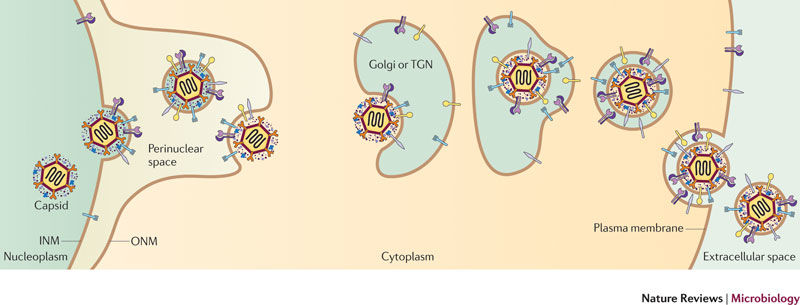
\includegraphics[width=\textwidth]{./viral_egress}
  \caption{Scheme of assembly and egress pathway of virus particles.
  After capsids are formed in the nucleus, they bud into the inner nuclear membrane (INM) (primary envelopment) to form an enveloped particle in the perinuclear space.
  These particles fuse with the outer nuclear membrane (ONM) (de-envelopment) and are released into the cytoplasm, leaving the envelope in the ONM.
  In the cytosol, capsids bind onto and bud into cytoplasmic membranes (secondary envelopment), and enveloped virions are secreted from cells (release).
  Figure from \cite{[2]}.}
  \label{fig:viral_egress}
\end{figure}

% \subsection{Early tegumentation assembly}
%
% %Tegumentation occurs during virion maturation.
% %Complex protein-protein interactions mediate tegument assembly.
% The intricate network of protein-protein interactions makes characterizing the precise function(s) of any individual protein difficult.
% The tegument composition changes during assembly and egress \cite[(reviewed in [2, 17])].
% The diversity of the tegument components raises the challenging question of how and where they are selected for incorporation into nascent virions.
% Overall, it is supposed that early coating with few tegument proteins occurs at the nuclear stage, some viral proteins are shed during nuclear egress, and other tegument proteins are acquired in the cytosol and during secondary envelopment \cite{[18]}.
% %One would suspect that
% %Early tegumentation may play a role primarily for virus egress
% %for directed transportation to the inner nuclear membrane, primary envelopment, de-envelopment and/or further unknown functions.
% %A recent study, using 3D single particle tracking, has shown that nuclear herpesvirus capsids do not use directed motility to reach the nuclear envelope.
% Using 3D single particle tracking, it was shown that nuclear herpesvirus capsids do not use directed motility to reach the nuclear envelope.
% Viral proteins work by changing the nuclear architecture to create space for capsid free diffusion rather than activating capsids for transport \cite{[19]}.
% After reaching the INM, budding occurs in order to transfer the capsids from the nucleus in the perinuclear space.
% The viral proteins pUL31 and pUL34 form the nuclear egress complex \cite{[20, 21]}, whose formation is crucial for budding \cite{[17, 22]}.
% pUL34 is a membrane protein attached to nuclear membranes, and upon complex formation also pUL31 accumulates at the nuclear rim \cite{[20]}.
% Both proteins are present on perinuclear capsids, but are then shed from the capsids and not existent on mature extracellular virions \cite{[17]}.
% Contradicting results were published if and which proteins of the mature tegument assemble at the capsids already within the nucleus.
% pUL36, pUL37, pUL41, pUL47, pUL48, pUL49, pUS3, ICP0, ICP4 are part of the tegument layer in mature virions and have been reported to partially localise within the nucleus.
% These findings have not been confirmed in other studies, and it is unclear whether these proteins associate with the nuclear capsids \cite{[5, 23\-32]}.
% Much evidence for early recruitment onto the capsids is found for pUS3, pUL36, pUL37, pUL41 and pUL49 which were identified in mature and perinuclear virions \cite{[18, 21, 33\-35]}.
% An increasing volume of evidence suggests that ICP0 and ICP4 are present on mature virions, but the intracellular compartment where this interaction occurs is open for debate [35\-39].
% Although they are not essential for nuclear egress [2], some of the putative early tegument proteins play a role in primary envelopment and/or de-envelopment [17, 40].
% Finally, whether any other tegument proteins also interact with nuclear capsids is presently unknown.

%\subsection{Single virus tracking}

% \subsection{Aims}
% Until now, no quantitative and systematic approach exists that makes use of fluorescence microscopy with all its capacity in single molecule imaging to investigate herpesvirus tegument assembly inside infected cells.
% Generally, it is assumed that tegumentation starts directly after capsid formation, but direct evidence from live-cell data is missing.
% In the current project, we aim to prove that the first steps of tegumentation take place inside the nucleus.
% Several viral proteins have been identified as possible candidates for early tegumentation.
% We plan to investigate their cellular location, attachment to nuclear capsids and functional roles.
% In order to achieve our goals, we choose an interdisciplinary approach at the interface of advanced fluorescence microscopy, virus biology and quantitative single particle tracking.
% The methods we propose will allow us for the first time to look at both virion assembly state and motion through the cell at the same time.
% Bringing together the expertise of myself and my former group (Prof. Kubitscheck, single particle tracking) and the hosting institution (Prof. Kaminski, SPIM and superresolution imaging) in collaboration with Dr. Crump (virus biology) will make this an ideal combination for success.
%
% Which tegument proteins are assembled at the capsids in the nucleus?
% Several proteins of the mature tegument of HSV-1 have been suspected to assemble at capsids within the nucleus.
% We intend to investigate the presence of the following candidates inside the nucleus of infected cells and upon nuclear capsids:
% 1)	pUL36 and pUL37:
% pUL36 (>330 kDa) is most probably required for stabilisation of the capsid vertex-specific component (CVSC, a complex of capsid proteins pUL17 and pUL25) of nuclear and cytoplasmic capsids [51].
% The CVSC promotes nuclear egress of DNA-filled capsids by direct interaction of pUL25 with pUL31 [52].
% pUL36 mediates binding of pUL37, the second-largest tegument protein [53].
% Both proteins appear to link capsid and tegument [2].
% 2)	pUL47, pUL48, and pUL49:
% These are the most abundant tegument proteins in the mature virion, and act as central organizers of the tegument [54].
% pUL48 is recruited to capsids mainly by interaction with pUL36 [55].
% All three proteins are not directly involved in nuclear egress, but might help to organize and stabilize the early tegument.
% 3)	pUS3 and pUL13:
% Both proteins are kinases.
% pUS3 and pUL13 may participate in primary envelopment by regulating the localization of the HSV-1 pUL31/pUL34 complex at the inner nuclear membrane [21, 56-59].
% However, pUS3 itself is not essential for primary envelopment, but rather plays a role in de-envelopment [21, 56, 57].
% 4)	ICP0 and pUL41: The proteins are regulators of viral transcription, and host/viral translation and immune response, respectively [5].
% ICP0 is probably recruited onto the capsids by pUL49 [38].
% Incorporation of pUL41 may be facilitated by interaction with pUL48, pUL49 and possibly pUL47 [54].
% First, we will systematically image the cellular distribution of the mentioned tegument proteins, especially during the phase of capsid assembly and egress.
% Hence, we will use dual fluorescent viruses with capsid (pUL35 or pUL25) and tegument proteins of interest tagged with auto-fluorescent proteins (mTurquoise, EGFP and mCherry), and perform live-cell time-lapse imaging.
% In order to obtain image sequences with high quality and detail, we plan to apply a resolution- and contrast-enhancing imaging technique such as structured illumination microscopy (SIM).
% We will further investigate the attachment of the tegument to single capsids.
% We intend to analyze co-localization of capsid and tegument proteins using two approaches: (a) single particle tracking in combination with image correlation [60], and (b) correlation between dual-colour motion trajectories [61].
%
% What are the functional roles of early tegument proteins?
%
% Recently, it was discovered that nuclear capsids are not actively transported, but move mostly by free diffusion [19].
% Hence, we assume that the most probable functions of early tegument proteins consist in organization and promotion of nuclear egress and availability as binding partners for other tegument or viral membrane proteins.
% After screening which of the investigated proteins attach to capsids, we will determine the location of the tegumented capsids with regard to the nucleus structure.
% We assume that the location of attachment is connected to the functional role.
% E.g. pUL36 is supposed to stabilize the complex of the capsid-associated proteins pUL17 and pUL25, hence very early attachment of this protein near the sites of capsid assembly would be expected.
% pUS3, ICP0 and pUL13 have been described to be involved in primary envelopment, thus we would suspect that assembly of these proteins would occur near the nuclear membrane.
% In order to analyze if putative early tegument proteins play a role in primary envelopment, we will examine if binding of tegument proteins provokes changes in capsid mobility due to membrane interaction.
% Co-localization with the nuclear egress complex (labelled pUL31 or pUL34 proteins) will provide further evidence about participation in primary envelopment.
% In a final step, we will investigate in which order tegument proteins bind to capsids what will give evidence about in vivo protein-protein interactions.

\section{Single Particle Tracking}

While optical imaging is generally limited to a resolution of \SI{\sim 250}{\nano\metre} nm by diffraction, sparse emitters can be localised with much higher precision by fitting a model function to their intensity distribution.
Tracking individual particles is an important tool for modern biology.
It has been used to study intracellular transport such as the movement of mRNA\cite{Spille2015a}; cell membrane dynamics\cite{Cognet2014} and more.
% Beneath the methods of super-resolution imaging, awarded by the Nobel Prize in chemistry in 2014, the principles of localisation microscopy are also applied in single particle tracking (SPT) as was shown already in early single molecule studies [41, 42].
%SPT is a real-time imaging technique that monitors the movement of individual particles and can provide information about dynamic behaviour within a biological system. %in a cellular context.
Many studies exist on inter and intra cellular viral trafficking
%virus trafficking between and inside cells
using single particle tracking \cite{(reviewed in [43])}.
%In general, more studies about the early stage of infection, virus entry and transport, exist than studies about the late stages of infection, virus assembly and egress.
Only a few and recent works exclusively probe the molecular egress pathway of herpesviruses.
Hogue \emph{et al.} \cite{[16]} used total internal reflection fluorescence (TIRF) microscopy to selectively visualise fluorescent Pseudorabies viruses near the plasma membrane and follow them during exocytosis.
Sandbaumhüter \emph{et al.} showed, by a motility analysis of fluorescent HSV-1, that directed transport of cytosolic capsids was dependent on both tegument proteins pUL36 and pUL37 \cite{[44]}.
Virus trafficking and how viruses penetrate the nucleus of a cell have also been studied using SPT \cite{Brandenburg2007}.
%The mentioned examples show that single-virus tracking can reveal detailed information about the dynamics of single viruses inside cells with high spatial and temporal resolution.

Due to a limited depth of field, particles tracked in a 3D volume tend leave the axial detection range.
%Data analysis then often relies on two dimensional projections of short trajectory fragments and might not accurately represent three-dimensional (3D) particle motion if the specimen structure is not isotropic \cite{[45]}.
Several technical approaches already exist to perform SPT in three dimensions \cite{[46-49]}.
%In the field of virology, very few studies have made use of the available 3D SPT techniques.% to date.
Orbital tracking in two planes was applied to track prototype foamy virus (PFV) in real-time inside cells \cite{[50]}, and a rotating, oblique light sheet and astigmatic detection were used to image and track viral capsids with high temporal and spatial resolution inside the cell nucleus \cite{[19]}.
%The new technical development opens up existing perspectives in studying herpesvirus assembly and egress in vivo.

%\section{Particle Tracking In Life Science}

%\subsection{Particle Tracking}

% Particle tracking is a relatively young but vital tool in modern quantitative biology and the field of bio-informatics.
% A particle can refer to anything that is particulate and is not exclusively large or small, circular or spherical etc.
% These techniques are very useful at numerically quantifying and detecting large population movements to discern general trends.
% For instance, pollen grain diffusion; a singular grain of pollen will be erratic and random whereas several hundred recorded paths will reveal a general diffusive trend through averaging.
% Particle tracking lends itself very heavily to the study of intracellular dynamics, answering important biological questions such as: viral infection movement\cite{Brandenburg2007}, intracellular membrane dynamics\cite{Chenouard2014}, genome maintenance, gene transcript\cite{Planchon2011} and more\cite{Cognet2014}.
%
% Particle tracking using light sheet microscopy is very relevant due to the high imaging speeds required to study particles that are both small and fast.
% Confocal microscopes suffer because they cannot temporally resolve particles; widefield microscopes suffer because they cannot provide three dimensional data; SPIM can offer both.

\subsection{Particle spatial localisation}

Particle tracking can be broadly described as a two stage process, spatial localisation then temporal localisation.
%The spatial localisation of a particle involves accurately marking where one or many particles are within an image.
%Humans are naturally able to do this as they have evolved to notice patterns and anomalies.
%Programming a computer to undertake this exercise was an early feat in the field of computer vision\cite{Crocker1996}.
Crocker \emph{et al.} deconstructed the problem into logical computable steps.
%Volumetric data is considered as singular images in two dimensions.
Each image is %then
corrected for any distortion or error from the digitation process as well a de-noising step. %as digitised video is inherently imperfect and may not be truly representative.
%Each image has a threshold found from an estimate of the background value of the image.
%This threshold removes substantial noise that would otherwise contribute to the final result.
Pixels with local maximum brightness are identified as \emph{candidate} particles and compete with other candidates within a pre-defined radius slightly larger than the expected size of the particle.
%\footnote{Methods since Crocker for a truly blind particle recognition have since been proposed but Crocker serves as a poignant historical but still relevant method of particle tracking using Computer Vision}
A centroid (centre of mass) fitting procedure is employed under the assumption that, %to a first order approximation,
spherical emitters can be well-defined by a Gaussian profile.
By fitting a Gaussian profile %and using tens of pixels to minimise error,
particulate positioning can be recorded with sub-pixel accuracy.
%The most common method of
Typically iterative least squares fitting is used %Gaussian fitting
due to its ease of implementation, speed, precision and robustness.% is iterative least squares fitting.

% \paragraph{Overlap}
%
% Crocker's method does not account for overlapping particle systems; experimental and computational methods are addressing this\cite{Serge2008}, but for the most part these cases are marked as rare outliers and typically rejected in particle tracking routines as samples are usually constructed with a sensible sparsity.


\subsection{Particle temporal localisation}

Temporal localisation refers to the assignment of linage to a particle.
%The reliab With fast imaging the reliable of such an assignment
Between frame 1 and 2, particulate identity is determined by minimising the sum global distance between particles at each time point.
By frame 3, momentum can be assigned the a particle as well to decrease the chance of two path identities being falsely merged or switched.
The same applies for acceleration and higher order speed derivatives, but with a lessening of overall significance.
The chance of a lineage being correctly assigned largely relies on the sampling rate of the imaging, with higher rates being favourable.
%particulate identify is determined from the closeness of

%The planet Pluto was originally discovered by Tombaugh in 1930 by comparing two images of the night sky a few hours apart.
%He would place an image in each side of his \textit{Blink comparator} and switch having his left or right eye open very quickly.
%With this he could intuitively notice trajectories of bodies in the sky.
%If his two images were taken years apart, his blink comparison metric would have been entirely chaotic.
%He chose a time span which ensured the that he could assign \textit{beyond reasonable doubt} likely trajectories between each image.

%The same principle applies to l
% When localising particles temporally, images of particle distributions need to be taken swiftly enough so that any change in particle position is small enough such that it can be judged as the same particle but in a different position at a  time later, \textit{beyond reasonable doubt}.
% Computationally this is achieved by assigning a global cost metric to the distance between particles which is then minimised to find the most likely solution of how particles in the first image have translated into the second image.

%\subsection{Single Particle Tracking}

\subsection{Light sheet single particle tracking}

Spille \emph{et. al.} proposed using light-sheet microscopy for tracking particles over long periods.
This was achieved by shifting their light-sheet and detection objective at each recorded frame such that the particle was repositioned to the centre of the sheet.
Alternatively, the entire sample could be relative to a static sheet.
Spille demonstrated this technique very successfully on a single molecule of mRNA (\(50 nm\)\cite{Spille2015a}) moving on the membrane of a nucleus\cite{Spille2015a} (see Figure \ref{fig:SPIMSPT}).
%
% demonstrated this technique very successfully on a single molecule of mRNA (\(50 nm\)\cite{Spille2015a}) moving on the membrane of a nucleus\cite{Spille2015a}.
%
% A very novel and exclusive way of full three dimensional particle tracking using SPIM has been proposed.
% By using a static light-sheet and an XYZ translator one can move a particle back into the FOV laterally if it drifts.
% Once the particle is re-localised, the encoded position on the \(z\) aspect of the stage is then equal to the position of the axial position of the particle by virtue of the repositioning.
% The \(x\) and \(y\) position are then derived using Crocker's centroid fitting from the resulting image accurately in post processing.
%
% This method vastly improves the lateral resolution of the SPIM system as well.
% Volumetric methods would limit the lateral resolution to half the beam waist, \(\sim 1 \mu m\), whereas this method is exclusively limited by the step size of the z translator (which can be very high resolution when using piezoelectric crystals) and one's ability to ensure the particle is precisely central within the excitation laser (which is then dependent on the particle size).
%
% SPIM's speed makes the technique very enticing as it is unrivalled for the purposes of particle tracking.


% This method could then be further improved using a tunable lens excitation, by tracking the position of the particle in \(x\) using the tunable lens and \(y\) by narrowing the trace of the scan mirror, the temporal and spatial resolution of single particle tracking could be vastly improved yet again.
% Z position information could also be encoded into the image by virtue of light beam intensity.
% By ensuring the particle is limited to half of the beam profile of the light sheet, then intensity of the particle would be proportional to a Gaussian curve z position.
% This method could prove to be faster, more accurate and less perturbing on the sample as mechanical motion would be removed.

\begin{figure}
	\centering
	\begin{subfigure}[b]{0.35\linewidth}
		\centering
		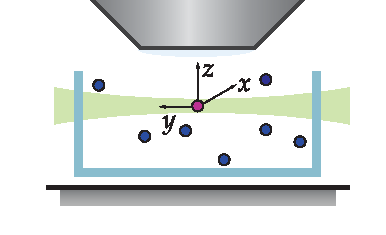
\includegraphics[width=0.8\linewidth]{Chapters/spt/Figs/PDF/tracking/1_piezo_track}
		\caption{Static particle localised in \(xy\)}
		\label{fig:SPIMSPT1}
	\end{subfigure}
        \hspace{0.05\linewidth}
	\begin{subfigure}[b]{0.35\linewidth}
		\centering
		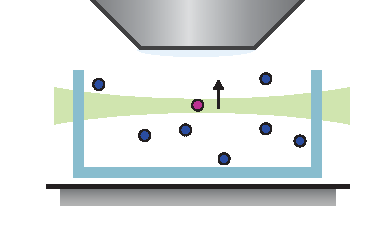
\includegraphics[width=0.8\linewidth]{Chapters/spt/Figs/PDF/tracking/2_piezo_track}
		\caption{Particle diffuses out of light-sheet}
		\label{fig:SPIMSPT2}
	\end{subfigure}
	\begin{subfigure}[b]{0.35\linewidth}
		\centering
		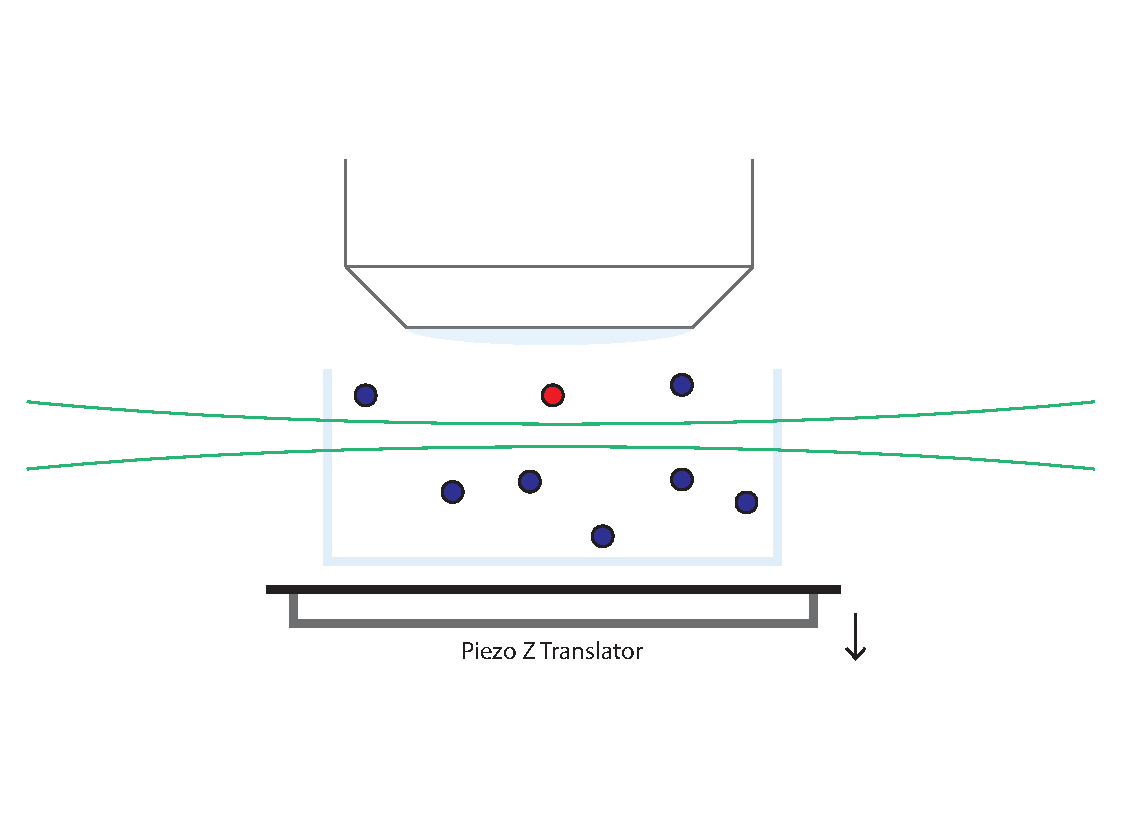
\includegraphics[width=0.8\linewidth]{Chapters/spt/Figs/PDF/tracking/3_piezo_track}
		\caption{\(z\) stage repositions so that particle is within light-sheet}
		\label{fig:SPIMSPT3}
	\end{subfigure}
        \hspace{0.05\linewidth}
	\begin{subfigure}[b]{0.35\linewidth}
		\centering
		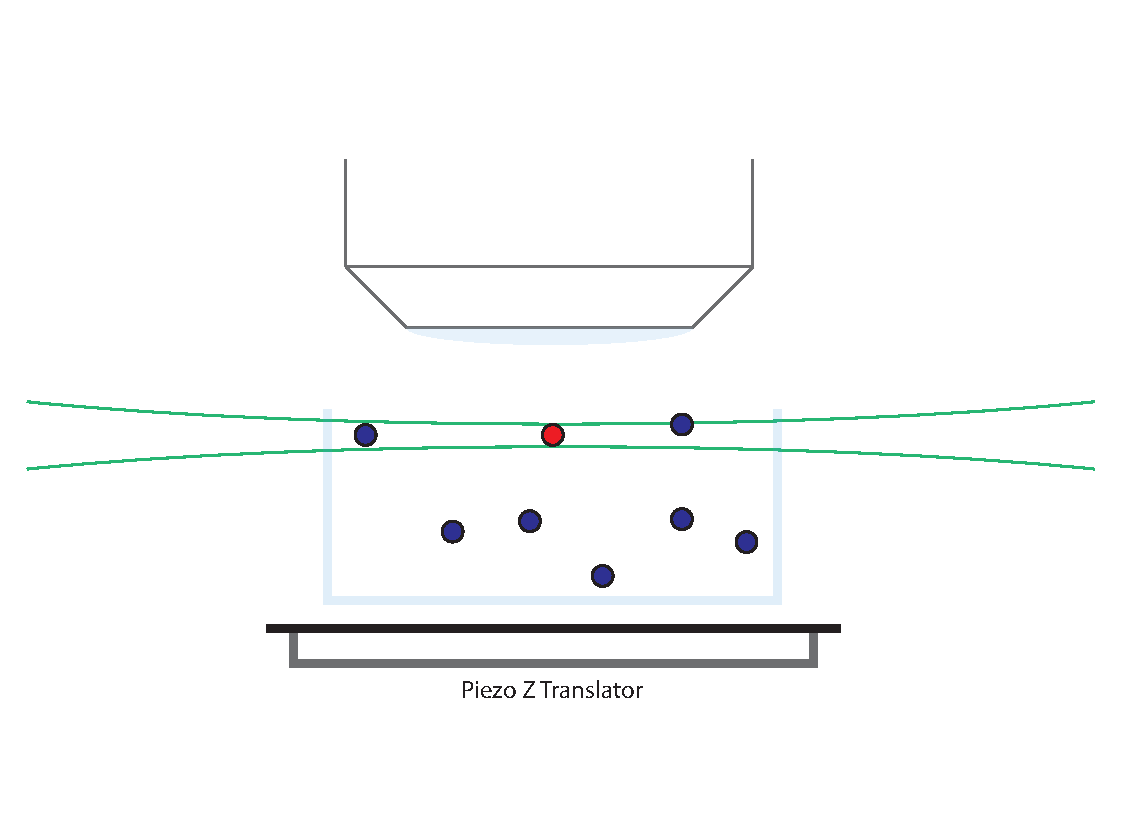
\includegraphics[width=1\linewidth]{Chapters/spt/Figs/PDF/tracking/4_piezo_track}
		\caption{Particle in light-sheet, \(z\) position recorded}
		\label{fig:SPIMSPT4}
	\end{subfigure}
	\caption{Routine to track particles three dimensionally using light-sheet.}
	\label{fig:SPIMSPT}
\end{figure}

\section{Astigmatic tracking}

%For axial particle tracking
To successfully reposition the light-sheet for axial particle tracking a %using light-sheet microscopy,
precise axial localisation, within the sheet, is needed.
%To know whereabouts within the light-sheet the particle is so that the light-sheet may coarsely reposition, a finer axial localisation is needed across the waist of the sheet.
Adding a weakly cylindrical lens within the detection optics will add astigmatism to the point spread function of the microscope.
The asymmetry in focal lengths in the imaging plane axes %of the imaging plane
means that along one axis the focal point will be offset axially compared to the orthogonal axis.
The result is that there in an overall axial asymmetry in the detection PSF, for point sources this allows axial position to be encoded in the recorded image.
This technique was used to great effect in dSTORM and PALM systems, which rely on the localisation of point emitters to create 3D volume super-resolution images \cite{}.
The range over which a cylindrical lens can axial encode is at most \SI{\sim 1}{\micro\metre}, before the non-linearity in the astigmatism becomes too great and the PSF is too blurred to fit computationally.

%Compare 2D guassian fitting ratio threatening
%\subsection{Fitting} %Guassian fitting
\subsection{Axial localisation}

Assuming an accurate localisation in 2D, the image of the point emitter is then localised axially.
With each of the methods presented here, a monotonic calibration volume of known distance is needed.

% Assuming an accurate localisation in 2D of a point emitter, the image of the astigmatic point emitter needs to
%
%  to then be compared to a calibrated sample.
% This is achieved by holding a point emitter and precisely moving it axially and recording an image stack.
% Typically the point emitter is held a gel-like phantom of the sample intending to be used.
% Once the calibration volume has been recorded, a trade-off between speed and accuracy is made.

\subsubsection{Gaussian fitting}

The ratio of the FWHM of the Gaussian along the major and minor axes will produce a calibration curve for axial position.
The major and minor axis sigma values are attained by Fitting a 2D Gaussian function to the rotated and and centered point image.
However, this technique is computational expensive and slow techniques to recover axial position is fitting a 2D Gaussian.
Attempting an iterative 2D Gaussian fitting in real-time is unrealistic with current computing capabilities, as such this technique is only useful in passive analysis of images already recorded.
%Talk about accuracy

\subsubsection{Template matching}

% Cros corelation
Cross-correlation requires no fitting step and scales in computational complexity with the image as $O(n^2)$. %TODO check this
As such using fewer pixels% are feasible
to recover axial position allows this technique to function in real-time.
The cross correlation of two signals returns a single value representing an unnormalised similarity of the two signals.
Provided the astigmatism is transitioning linearly, a cross-correlation for every image in the calibrated stack may not be needed.
By using all the images in the calibration stack, the computational time increases by the half the number of axial images in that stack.
The ratio of the the cross correlation of two images spaced axially and equally about the focal centre of the stack will give an estimate of particle position
This estimate is sufficient for real-time results; and provided the images of the point-emitter are recorded, a more accurate axial localisation step can be applied in post-analysis.
The discrete cross-correlation function:
\begin{align}
(f \star g)[n]\ \stackrel{\mathrm{def}}{=} \sum_{m=-\infty}^{\infty} f^*[m]\ g[m+n]
  %I_{\text{Cross correlation} =
  %(f \star g)[n]\ \stackrel{\mathrm{def}}{=} \sum_{m=-\infty}^{\infty} f^*[m]\ g[m+n].
\end{align}
Similarly the covariance of the calibration an image or volume can be used, though the computational complexity is lower again.
%Talk about errors n shit
\begin{align}
  \operatorname{cov}(X,Y) &=\frac{1}{n}\sum_{i=1}^n (x_i-E(X))(y_i-E(Y)) \\
 &= \frac{1}{n^2} \sum_{i=1}^n \sum_{j=1}^n \frac{1}{2}(x_i - x_j)\cdot(y_i - y_j)
\end{align}

\subsection{Simulations}
To verify that single particle tracking in light-sheet microscopy was possible, the diffusion of a single diffraction limited particle was simulated \emph{in silico} (see Figure \ref{fig:diffusion}).
To create the simulation, the particle was modelled to take a random walk of time steps $dt$ across a single imaging exposure of \SI{40}{\milli\second}.
This simulated how the particle would appear to move within the light-sheet.
The intensity of the final image of a particle was attenuated according to the Gaussian intensity of the light-sheet axially($z$) and laterally ($x,y$) as per:

\begin{align}
  w_0 &= 1.4 \lambda \frac{ \text{NA}}{n}\\
  w(y) &= w_0 \sqrt{1+\left(\frac{y}{y_R}\right)^2}\\
  y_R &= \frac{\pi w_0^2}{\lambda}\\
  I(x,y,z) &= I_0 \left(\frac{w_0}{w(y)}\right)^2 e^{\left(-2\frac{z^2}{w(y)^2}\right)}
\end{align}

Where $w_0$ is the beam waist; NA is the numerical aperture of the excitation objective, $n$ is the refractive index of glass; $\lambda$ is the wavelength of excitation light; $y_R$ is the Rayleigh length and $w(y)$ is the beam waist through $y$.


% \begin{figure}
% 	\centering
% 	\begin{subfigure}[b]{0.35\linewidth}
% 		\centering
% 		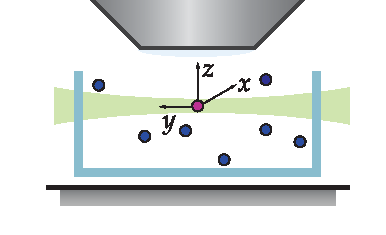
\includegraphics[width=0.8\linewidth]{Chapters/spt/Figs/PDF/tracking/1_piezo_track}
% 		\caption{Static Particle localised in \(xy\)}
% 		\label{fig:SPIMSPT1}
% 	\end{subfigure}
% 	\begin{subfigure}[b]{0.35\linewidth}
% 		\centering
% 		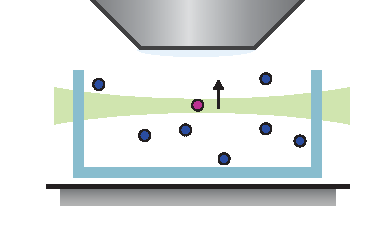
\includegraphics[width=0.8\linewidth]{Chapters/spt/Figs/PDF/tracking/2_piezo_track}
% 		\caption{Particle diffuses out of light sheet}
% 		\label{fig:SPIMSPT2}
% 	\end{subfigure}
% \end{figure}

\begin{figure}
  \centering
  \begin{subfigure}[b]{0.8\linewidth}
    \centering
    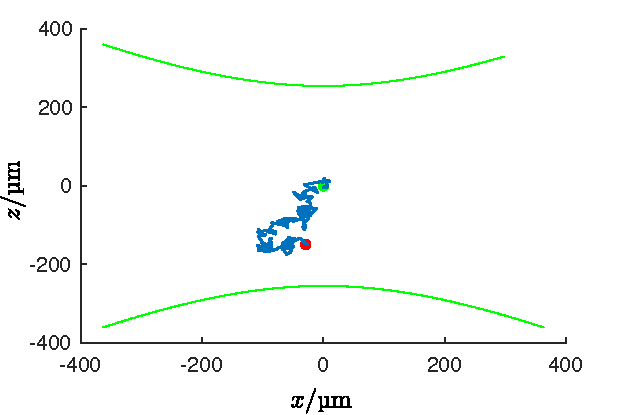
\includegraphics{./simulation/size_view_diffusion}
    \caption{Side-view}
    \label{fig:size_view_diffusion}
  \end{subfigure}
  \begin{subfigure}[b]{0.8\linewidth}
    \centering
    %%!tikz editor 1.0
\documentclass{article}
\usepackage{tikz}
\usepackage[graphics, active, tightpage]{preview}
\usepackage{graphicx}
\usetikzlibrary{positioning}

\PreviewEnvironment{tikzpicture}

%!tikz preamble begin

%!tikz preamble end


\begin{document}
%!tikz source begin
\begin{tikzpicture}
  \node (img)  {\includegraphics{view3_diffusion}};
  \node[below=of img, node distance=0cm, yshift=1cm] {$xy$ plane};
  \node[left=of img, node distance=0cm, rotate=90, anchor=center,yshift=-0.7cm] {$z$ axis};
 \end{tikzpicture}
\end{document}

    %\includegraphics{./simulation/diffusion_3d}
    %\includegraphics{./simulation/diffusion_3d.pdf}
    \caption{3D view}
    \label{fig:diffusion_3d}
  \end{subfigure}
  \caption{Simulations of a single particle diffusing within a light-sheet with a viscosity of 25\% glycerol in water}
  \label{fig:diffusion}
\end{figure}

\section{Motion induced astigmatic axial localisation error}\label{sec:spt_maths}

It was demonstrated in the computational simulations that a particle moving in a real system will demonstrate a motion blur unique to having astigmatism.
A single particle moving quickly in $xy$ will appear to stretch and the localised position of the particle will be the average of the start and end position.
With astigmatism, the image of particle does not vary linearly with the distance the particle has travelled axially during that epoch.
%\subsubsection{Astigmatism}
This response was modelled % using a false
using
a false astigmatism %was used, %added to the simulation,
to emulate an approximate response of the system.
A Gaussian was convolved with the single point in space, with the assumption that the depth of field of the detection objective was longer than the width of the light-sheet and that intensity across the sheet was uniform;
the latter assumption is invalid, but a varying intensity only controls the SNR across the sheet.
A Gaussian function being used to model a particle is a valid assumption as Gaussian models are used in the fitting process for localisation from the pixel data.

To astigmatically narrow the Gaussian as the particle moved through $z$ the standard Gaussian equation of:
\begin{align}
  f(x,y) &= e^{-\frac{x^2 + y^2}{\sigma^2} }
\intertext{was modified to use a simple model of astigmatism %.}
%\intertext{Featuring an assumed linear astigmatism where $c$ is the bias value to create a minimum width of the particle the diffraction limited spot size and $k$ is the degree of astigmatism featuring.
%In real optical systems astigmatism is non-linear but assumed to be linear for short distances from the focal plane.}
%\intertext{%To create a simple model of astigmatism we
by assuming assume that $\sigma$ depends on $z$ such that:}
\sigma(z) &= kz + c
\intertext{Where $k$ is an arbitrary degree of astigmatism and $c$ is the particle size when there is no astigmatism.
We can then redefine $k$ in terms $a$, where $a$ is a function of $c$ and $L_{\text{end}}$, with $L_{\text{end}}$ being the distance the particle will be when
the Gaussian is $\frac{1}{a}$ narrower:}
k & = \frac{a c}{L_{\text{end}}}
\intertext{The negative gradient relationship then holds for the orthogonal dimension to give a full 3D model:}
f(x,y,z) &= e^{-\frac{x^2}{kz+c} +\frac{y^2}{-kz+c} }
\end{align}
\begin{figure}
  \centering
  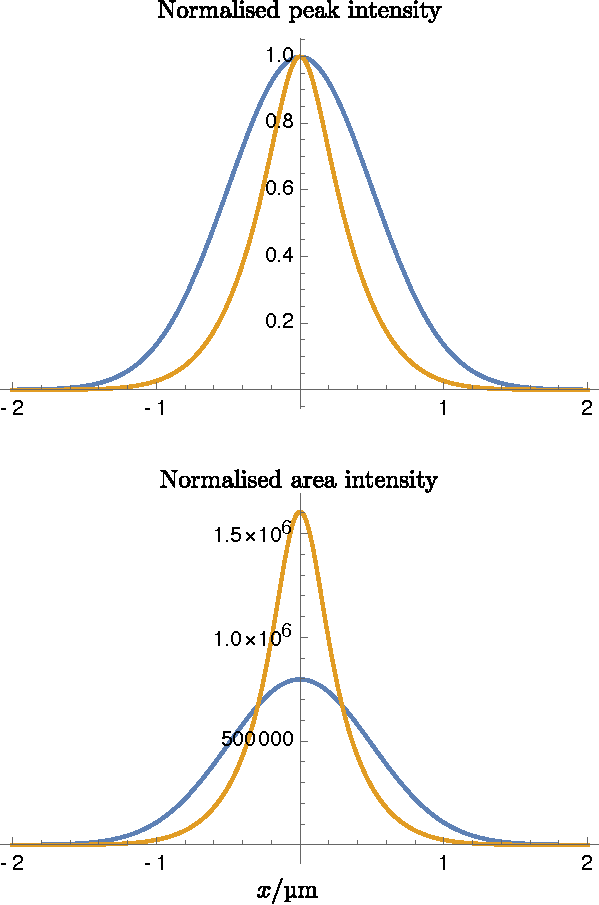
\includegraphics{./mathematica/guassians}
  \caption{a) Expected versus reality PSF profile of a particle using normalised peak intensity, a weaker model for astigmatism
  b) Uses normalised area of the Expected and Reality PSFs for a more accurate model of astigmatism}
  \label{}
\end{figure}
%By using a simple one dimensional model of astigmatism acting on Gaussian the motion blur due to astigmatism can be quantified analytically.
%\subsection{Model}
%\begin{align*}
  %A Gaussian function being used to model a particle is likely a valid assumption as Gaussian functions are in turn used in the fitting process for localisation of the pixel data:}
  %&e^{-\frac{x^2}{2 \sigma^2}}
%\end{align*}
\begin{align}
\intertext{To make calculations tractable, all modelling was considered in $xz$ as the effect of astigmatism in $y$ is independent.
%\intertext{
By normalising the Gaussian model, we simulate that an equivalent number of photons are being emitted by the particle, this allows the Expected and Reality PSFs to be compared.
The Expected PSF is defined such that no motion blur is considered:}
\hat{\text{PSF}}_{\text{Expected}} &= \frac{1}{\sigma(z) \sqrt{2\pi}}e^{-\frac{x^2}{2 \sigma(z)^2}}\\
{\text{PSF}}_{\text{Expected}} &= e^{-\frac{x^2}{2 \sigma(z)^2}}
\end{align}
\begin{align}
 \intertext{Assuming that the particle moves a distance $L$ with uniform speed and uniform emission of photons en-route, integrating the Expected PSF gives the Reality PSF as subject to motion blur:}
\hat{\text{PSF}}_{\text{Reality}} &= \frac{1}{L}\int_{0}^{L}\frac{1}{\sigma(z) \sqrt{2\pi}}e^{-\frac{x^2}{2 \sigma(z)^2}} \mathop{dz}\\
&= \frac{{L_{\text{end}}} \left(\text{Ei}\left(-\frac{x^2}{2 c^2}\right)-\text{Ei}\left(-\frac{{L_{\text{end}}}^2 x^2}{2 c^2 ({L_{\text{end}}}+a L)^2}\right)\right)}{2 \sqrt{2 \pi } a c L} \\
\intertext{The integral has to be scaled by $\frac{1}{L}$ as integrating a function over $0 \to L$ will scale the total area by L. The resultant function is then by comparable with $\text{PSF}_{\text{Expected}}$.}
{\text{PSF}}_{\text{Reality}} &= \frac{2 c (a L+L_{\text{end}}) e^{-\frac{L_{\text{end}}^2 x^2}{2 c^2 (a L+L_{\text{end}})^2}}}{2 a c L} \\
&+ \frac{L_{\text{end}} x\sqrt{2 \pi }\text{Erf}\left(\frac{ (L_{\text{end}} x)}{\sqrt{2} (a c L+c L_{\text{end}})}\right)}{2 a c L} \\
&+ \frac{L_{\text{end}} \left(2 c e^{-\frac{x^2}{2 c^2}}+\sqrt{2 \pi } x \text{Erf} \left(\frac{x}{\sqrt{2} c}\right)\right)}{2 a c L}
\end{align}
%Gaussian, approximation of a particle
%PSF expected, width linearly depependent on z
%PSF reality, integral between 0 and L, scaled by L

\subsection{Area analysis}

For Guassian-like functions the total area under the curve is proportional to $\sigma(z)$, so by comparing the area covered by the expected and real PSFs a valid measure of error could be obtained.
This analysis does not work for normalised PSFs as the area is unity in each case, as such the unnormalised model was used.
Using an unnormalised function was still valid as the area was only being used as a proxy for finding a measure of the width of the PSF being interrogated.
\begin{align*}
  \int_{-\infty}^{\infty} \text{PSF}(x,...)_{\text{Expected}} \mathop{dx} &= \frac{\sqrt{2 \pi }}{\sqrt{\frac{1}{\left(\frac{a c L}{L_{\text{end}}}+c\right)^2}}}\\
  \int_{-\infty}^{\infty} \text{PSF}(x,...)_{\text{Reality}} \mathop{dx} &=\sqrt{\frac{\pi }{2}} \left(\frac{2 (a L+L_{\text{end}})}{a L \sqrt{\frac{L_{\text{end}}^2}{c^2 (a L+L_{\text{end}})^2}}}-\frac{2 L_{\text{end}}}{a \sqrt{\frac{1}{c^2}} L}+c \left(-\frac{a L}{L_{\text{end}}}-2\right)\right)
\end{align*}
\begin{align*}
  \text{Error} &= \frac{\int_{-\infty}^{\infty} \text{PSF}(x,...)_{\text{Expected}} \mathop{dx} - \int_{-\infty}^{\infty} \text{PSF}(x,...)_{\text{Reality}}\mathop{dx}}
  {\int_{-\infty}^{\infty} \text{PSF}(x,...)_{\text{Expected}} \mathop{dx} + \int_{-\infty}^{\infty} \text{PSF}(x,...)_{\text{Reality}}\mathop{dx}} \\
  &= \frac{2. \left(-\frac{2 L_{\text{end}}}{a L \sqrt{\frac{L_{\text{end}}^2}{c^2 (a L+L_{\text{end}})^2}}}+\frac{2 L_{\text{end}}}{a \sqrt{\frac{1}{c^2}} L}+c \left(\frac{a L}{L_{\text{end}}}+2\right)\right)}{\frac{2 (2 a L+L_{\text{end}})}{a L \sqrt{\frac{L_{\text{end}}^2}{c^2 (a L+L_{\text{end}})^2}}}-\frac{2 L_{\text{end}}}{a \sqrt{\frac{1}{c^2}} L}+c \left(-\frac{a L}{L_{\text{end}}}-2\right)}
\end{align*}

\begin{figure}
  \centering
  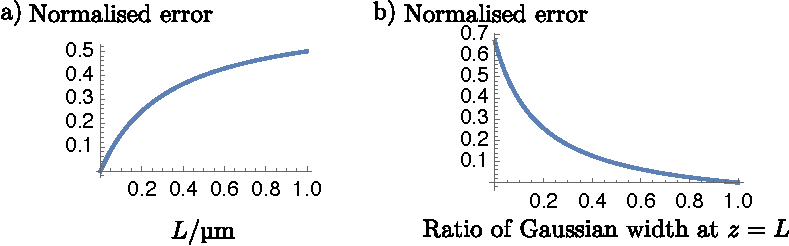
\includegraphics{./mathematica/area_analysis}
  \caption{
  a) Error was plotted against distance the particle travels in a single epoch%TODO
  b) The degree of astigmatism $k$ was reframed such that it a substitute parameter represented the ratio of the width of the Gaussian at $z=0$ and $z=L$.
  This graph shows that as the ratio approaches unity the error due to astigmatic smearing becomes $0$.
  However, when the ratio of the widths approaches 0, the error does not approach infinity as would be expected.
  }
  \label{fig:area_analysis}
\end{figure}

\begin{align*}
  \intertext{The above equation details how much error, in width, the astigmatism is expected to accrue over a length $L$. This length $L$ may be computed from the three dimensional diffusivity of a small particle from the diffusivity $D$:}
  D = \frac{kT}{6 \pi \mu r}
  \intertext{Where $k$ is Botlzmann's constant, $T$ is temperature, $\mu$ is the viscosity of the medium, $r$ is the radius of the particle, from $D$ the average distance of diffusion $w$ can be computed:}
  w^2 = q_i D t
  %\intertext{}
\end{align*}
Where $q_i$ is the dimensionality of the diffusion and $t$ is the time elapsed.
By setting the parameters to realistic world values: $T=\SI{298}{\kelvin}$;
$\mu=\SI{0.002}{\newton\second\per\meter\square}$;
$k = \SI{1.3806e-23}{\meter\square\kilo\gram\per\square\second\per\kelvin}$;
$c = r = \SI{100}{\nano\meter}$;
$a = \frac{1}{5}$;
$L_{\text{end}} = \SI{0.5}{\micro\meter}$;
an average axial position error of \textbf{25.7\%} is observed.
% The above expression only considers $x$ and $z$ for simplicity of calculation.
% The ratio of the linear Gaussian-like function and the expected ($e^{-\frac{x}{2kL+c}^2}$) Gaussian is integrated over all space to provide an error value as a function of $L$ which is the distance the particle has traveled.
% The model presented here also does not take into consideration the variation of illumination across the light-sheet %TODO DISUCSS.
%
% Provided the smeared result is still Gaussian like, finding the FWHM will give an analogue of what a computer will fit.
% Doesn't resolve
% Taylor expansion
%
% It is assumed that a particle will not diffuse sufficiently quickly as to cause a deviance to the PSF then used to characterise the location of the particle.
% However, assuming the worst case of a particle diffusing in a straight trajectory (in the 2D case) the localised position of the particle will be the average of the start and end positions of the particle.
% This smearing leads to very non-Gaussian PSFs when diffusivity is high (Figure \ref{fig:})
% Worse still, the PSF response of the particle is also axially dependent when using an astigmatic lens.
% using the linear approximation of a linear astigmatic-like Gaussian and assuming the worst case of a particle diffusing directly up, an analytical solution for the error incurred may be imputed:
%
% \begin{align}
% %  {\int_{-\infty}^{\infty} \frac{\int_{0}^{L} e^{-\frac{x}{2(kz+c)}^2} dz}{e^{-\frac{x}{2kL+c}^2}} \mathop{dx}} \\
%   \text{PSF}_{\text{Expected}} &= \int_{0}^{L} e^{-\frac{x}{2(kz+c)}^2} dz \\
%   \text{PSF}_{\text{Reality}} &= e^{-\frac{x}{2kL+c}^2} \\
%   \text{Error} &= 2 \int_{-\infty}^{\infty} \frac{ |\text{PSF}_{\text{Expected}} - \text{PSF}_{\text{Reality}}|}{\text{PSF}_{\text{Expected}} + \text{PSF}_{\text{Reality}}} \mathop{dx} \\
%   \intertext{This integral does not compute, so instead relative areas beneath the Gaussians were considered}
%   \text{Error} &= 2 \frac{|\int_{-\infty}^{\infty} \text{PSF}_{\text{Expected}} - \int_{-\infty}^{\infty} \text{PSF}_{\text{Reality}}|}{\int_{-\infty}^{\infty} \text{PSF}_{\text{Expected}} + \int_{-\infty}^{\infty} \text{PSF}_{\text{Reality}}} \mathop{dx} \\
%   & = 2 \frac{\left(\frac{2 \sqrt{\pi }}{\sqrt{\frac{1}{(c+k L)^2}}}-\sqrt{\pi } (2 c+k L)\right)}{\sqrt{\pi } (2 c+k L)+\frac{2 \sqrt{\pi }}{\sqrt{\frac{1}{(c+k L)^2}}}}
% \end{align}
%
% Which is related to the diffusion constant
% The result of integrating over all space returns a function several infinities, so a smaller window is considered.
% Using a factor of $c$ is valid as $c$ governs the minimal width of the PSF.
% \begin{figure}
%   \centering
%   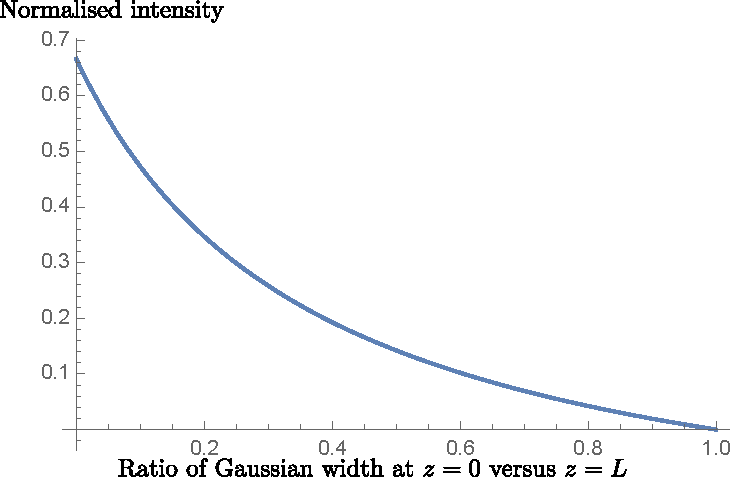
\includegraphics{./mathematica/Expected_versus_reality_error}
%   \caption{The degree of astigmatism $k$ was reframed such that it a substitute parameter represented the ratio of the width of the Gaussian at $z=0$ and $z=L$.
%   This graph shows that as the ratio approaches unity the error due to astigmatic smearing becomes $0$.
%   However, when the ratio of the widths approaches 0, the error does not approach infinity as would be expected.
%   }
%   \label{fig:Expected_versus_reality_error}
% \end{figure}
%
% \begin{figure}
%   \centering
%   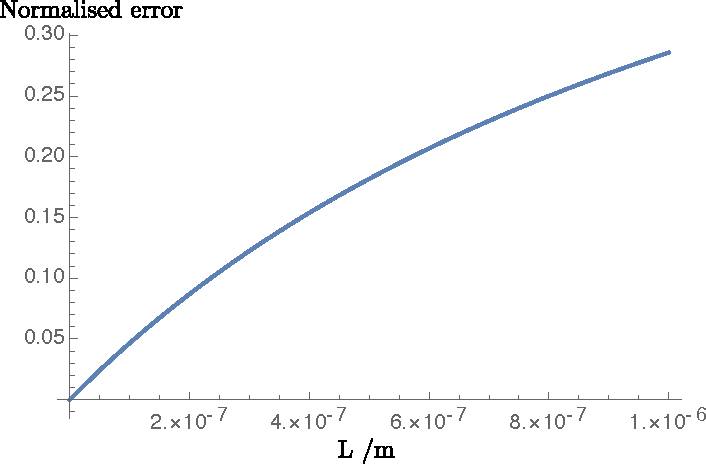
\includegraphics{./mathematica/Error_vs_L}
%   \caption{}
%   \label{fig:Error_vs_L}
% \end{figure}
%
% %!tikz editor 1.0
\documentclass{article}
\usepackage{tikz}
\usepackage[graphics, active, tightpage]{preview}
\usepackage{graphicx}
\usetikzlibrary{positioning}

\PreviewEnvironment{tikzpicture}

%!tikz preamble begin

%!tikz preamble end


\begin{document}
%!tikz source begin
\begin{tikzpicture}
  \node (img)  {\includegraphics{view3_diffusion}};
  \node[below=of img, node distance=0cm, yshift=1cm] {$xy$ plane};
  \node[left=of img, node distance=0cm, rotate=90, anchor=center,yshift=-0.7cm] {$z$ axis};
 \end{tikzpicture}
\end{document}

% \begin{figure}
%   \centering
%   %\includegraphics{/path/to/figure}
%   \caption{A single diffusing in medium was simulated using near native cellular conditions to establish the viability of particle tracking in the microscope.}
%   \label{}
% \end{figure}
% \subsubsection{PSF Smearing}
% Idealsied particle looks like
% Actual particle will have a smearing effect so you will always assume you've got less far in xyz
% When considers
\section{Results}

\subsection{Cellular imaging}

As a proof of principle, virally infected HeLa cells were mounted and imaged using the modified light-sheet microscope.
%\subsubsection{Mounting}
%As seen in chapter X mounting on flat glass is difficult.
%Cell culture requires a buffered medium, with most commercial solutions involving atmospheric control
The cells were infected with HSV-1 expressing tegument proteins fused to fluorescent proteins (VP26-mTurquoise, VP1/2-dtTomato, VP16-cYFP).
%The infected cells were %infected with
%HeLa cells were
%mounted on clean \SI{25}{\milli\metre} $\times$ \SI{25}{\milli\metre} coverslips.
Trypsin was used to help lift cells in culture into solution and was left to act for \SI{3}{\minute}.
10\% Foetal Bovine Serum (FBS) was added to deactivate the Trypsin as it is a protease enzyme and will further degrade the cells.
Coverslips were submerged in the cellular solution and left to adhere and culture on the glass.
3\% paraformaldehyde was used to fix cells for the preliminary visualisation experiments.
The glass coverslips were mounted in the custom imaging chamber discussed in Chapter \ref{chapter:chamber} for light-sheet imaging.

%The some viral tugment proteins (VP26, VP1-2, VP16) for

\begin{figure}
	\centering
	\begin{subfigure}[b]{0.7\linewidth}
    \centering
    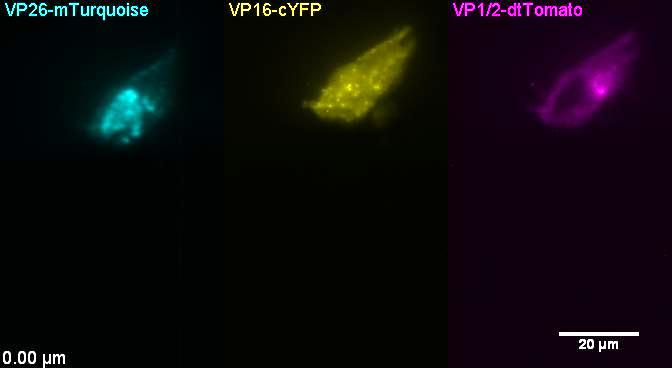
\includegraphics[height=5cm]{/calibration/three_colour_slice}
    \caption{Separate colour channels}
    \label{fig:merged_slice}
	\end{subfigure}
	\begin{subfigure}[b]{0.2\linewidth}
    \centering
    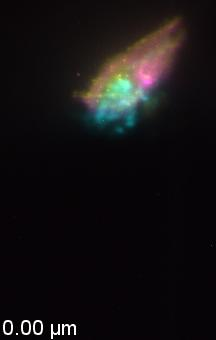
\includegraphics[height=5cm]{/calibration/merged_slice}
    \caption{Merged}
    \label{fig:three_colour_slice}
	\end{subfigure}
	\caption{HSV-1 viral tegument proteins volumetrically imaged in fixed cells using a light-sheet microscope.}
	\label{fig:virus_image}
\end{figure}

\section{SPT using SPIM}

The secondary optical relay was set to \SI{2.5}{\times} magnification, giving \SI{62.5}{\times} at the sample plane, to unsure the camera was Nyquist limited so that there were sufficient pixels available to observe astigmatism on a single particle.
The weakly cylindrical lens ($f = \SI{1}{\metre}$) was inserted in between the secondary relay and the camera unit at \SI{40}{\milli\metre} away from the aperture of the camera.
%This was found empirically to be sufficiently astigmatic by eye.
The cylindrical lens was inserted in between the camera and the tube lens as adding the cylindrical lens in an infinity space would have amplified the astigmatic effect (to beyond usable), and disabled any tuning of the astigmatism through positioning.

% %Placing a very long focal length cylindrical length
%
% ; for this system presented here, that would mean using a custom very long focal distance lens. %amplifies the effect and so a custom lens would have been needed.

\begin{figure}[h]
  \centering
  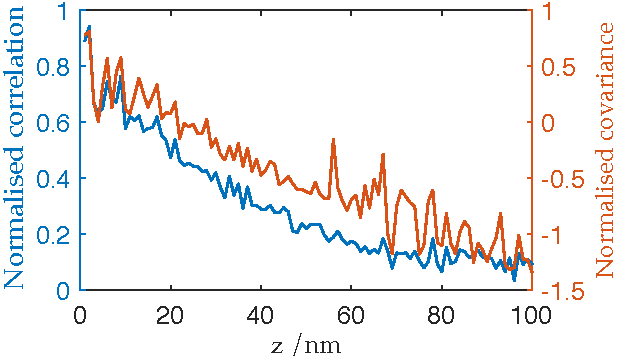
\includegraphics{./calibration/Calibration.pdf}
  \caption{Curves showing calibration between axial depth within the light-sheet and template matched cross-correlation (blue) and covariance (orange)}
  \label{fig:SPT_Calibration}
\end{figure}

For calibration of the axial particle tracking, an agarose gel of beads was imaged with the objective and the light-sheet synchronously iterated through small axial steps.
Moving the stage would have better emulated how a particle would appear, however, the mechanical resolution and hysteresis of the translation stage made this infeasible.

To compare the quality of the calibration, %The calibrations
the curves were linearly regressed, see Table \ref{tab:linear_calibration}.
%When fitting a linear regression %we find that
It was shown that using cross correlation provides a more linear curve calibration.
However there is a lower residual sum of squares, meaning co-variance may reduce the error in fitting. %due there being
As the neither of the calibration curves are obviously linear, a linear regression may not be the best metric for comparison; however, there is no model for how the system should respond and so using another function would be guess work.
Empirically, the calibration curve for correlation looks less variant than when using covariance, suggesting a linear fit is not sufficient.

\begin{table}[h]
\centering
\caption{Table of regressional analysis for calibration curves in Figure \ref{fig:SPT_Calibration}.
\label{tab:linear_calibration}
RSS: Residual sum of squares; $R^2$: Coefficient of determination; RMS: Root mean square}
  \begin{tabular}{lccc}
    \toprule
    Metric & RSS & $R^2$ & RMS \\\midrule
    Covariance & 0.633 & 0.8569 & 0.08037 \\
    Cross-correlation & 2.984 & 0.8904 & 0.08037 \\
    \bottomrule
  \end{tabular}
\end{table}

%TALK HERE ABOUT $R^2$ AND VARIANCE
% %Covar:
% SSE: 0.633
% R-square: 0.8569
% Adjusted R-square: 0.8554
% RMSE: 0.08037

%% X correlation
% SSE: 2.984
% R-square: 0.8904
% Adjusted R-square: 0.8893
% RMSE: 0.1745
%It was shown that a calibration

\section{Conclusions}

It was shown that the inverted light-sheet system as described in this work is capable of axially localising diffraction limited particles.
This was demonstrated experimentally using static sub-diffraction limit particles with a view to applying the same techniques to dynamic particles.
It was also shown that dynamic particles within when tracked astigmatically are susceptible to a localisation error on the order of 25 \% given standard imaging and biological conditions.
This was demonstrated on a model system analytically and could be used in other systems for calculations.

The detection objective used in the light-sheet system was victim to significant spherical aberration.
The spherical aberration was addressed using a bespoke tool to manually rotate the correction collar on the objective lens; this then lead to dramatic coma effects which had otherwise been masked by spherical aberration.
The latter aberration could not be corrected for which made Gaussian fitting in feasible for axial localisation.
However, template matching techniques did still produce a viable calibration curve that could be used, with cross-correlation being the more reliable reporter.

%which is why the cross-correlation of the current signal to the top and bottom templates produced a less variant calibration curve.

\subsection{Future work}

It was also shown that a Nyquist limited cellular image could also be acquired using this system.
By using a CO2 free buffer, such as HEPES, HeLa could be imaged in this system for long enough to observe viral egress within a live cell.
The next step for particle tracking would be to observe single particles diffusing in a viscous medium that acts as an analogue for the cell.
Once both of these have been demonstrated, SPT of viral egress from a live cell may be achieved.

%Would've been good to calibrate more than one colour?
\subsubsection{Neural networks} %Need to try training using this using convolutional neural networks
%Also possible to

In this work, the techniques presented for localising particles, in an astigmatic system, rely on a singular calibrated point emitter, the template.
A population of point-emitters with known axial positions would help mitigate potential axial localisation errors.
It is possible to align multiple calibration volumes and create an averaged or model calibration volume to work with, though this method relies heavily on the sub-pixel alignment step to reduce error.

Training a neural network could be a more robust approach.
Neural networks take multiple inputs and produce a single output based on a back propagation step which helps determine the weightings on the \emph{neurons} in the hidden layer or layers.
Convolutional neural networks work in a similar fashion except that the weightings are image convolution steps; by using convolution steps the overall size of the neural network needed reduces making image recognition possible.
By training a neural network on a given input segmented input image, with the known output of axial position, a fast and accurate machine for producing axial localisations could be utilised.
Neural networks are also computationally inexpensive as most of the effort put in occurs during the training step.

%Cancer, \textit{in vivo studies} have "progress[ed] in monitoring neurodegenerative disease pathobiology"\cite{Hoffman2005}
%3D imaging in \textit{in vivo} is desirable and currently use complimentary techniques (microCT) to create 3D.

% \subsubsection{Neuro-degenerative Disease}
%
% %Tau proteins misfold to cause neurofibrillary tangles.
%
% Current Alzheimer's disease models suggest that Amyloid beta fibrils elongate creating Amyloid plaques.
% These plaques then pathologically cause an over production of tau in the first affected neuron.
% This over production in the first neuron quickly produces toxic levels of tau which propagate into neighbouring neurons, causing a cascade neuronal degeneration\cite{King2002}.
%
% Mechanisms for AD are not fully understood but tau protein misfolding is expected to play a role in the pathology\cite{LaFerla2008}.
% Our group has shown that extracellular tau proteins cause the endogenous over-production of tau proteins\cite{Michel2014a}.
% The group has begun to observe tau propagation in axons two dimensionally.
% Observing the movement of tau proteins between neurons three dimensionally would perhaps reveal the mechanisms by which tau pathology neurodegeneration occurs, more specifically how extracellular tau proteins originated.
% It is hypothesised that stress impact may be a cause of the secretion of tau proteins causing the degeneration of other neurons\cite{Gavett2011,Patterson2014a}.
% An \textit{in vivo} study in a live animal model being impacted could verify this using light sheet particulate tracking.
%
% It is possible that tau proteins move too quickly to be successfully tracked.
% In our group Tau proteins have been monitored to move between neurons via axons at a rate of \SI{480}{\micro\meter} per 20 minutes or 0.4 um per second.
% A standard confocal image exposure is on the order of 2 to 3 seconds, meaning a tau protein could displace during the image acquisition by \SI{1.2}{\micro\meter}.
% This movement during exposure could lead to a tau protein appearing to be of the order microns, whereas in fact it is of the order tens of nanometres.
% Light sheet technology can image \SI{300}{} times faster and so a propagating tau protein would only move \SI{4}{\nano\meter} during an acquisition, less than the size of the protein and so an acceptable error.
% Most importantly, tau is of comparable size to mRNA which has already been successfully tracked within a live cell using light sheet SPT\cite{Spille2015a}.

% \subsection{Virus Trafficking}
%
% Virus particles are of the same length scale as mRNA and tau proteins and so can also be tracked using light sheet SPT.
% Viruses reproduce by exploiting cell structure.
% A virus particle will interact with the cell membrane either singularly or in a plaque to release the contents of the virus inside the cell.
% Proteins are released to suppress the immuno-response and enable suitable conditions for the viral genome move into the cell.
% Once inside, the virus moves to areas within the cytoplasm or nucleus and begins replication.
% Replicated virons then leave the cell and the cycle continues.
% Individual virus particles may follow a multitude of different paths or even fails completely during infection.
% By tracking viral infection at the single virus level observers can deconstruct the dynamics of virus-cell interactions.
%
% There are several challenges in tracking virus particles.
% Firstly, viruses are small, varying from 20 to 200 nm, sub-diffraction limit. %Their speed may also be a factor %todo.
% Virus labelling is also difficult due to its size and nature.
% Fluorescent probes are comparable to the size of the virus and so can hinder infectivity.
% Proximity of the fluorescent probes due to virus size can also cause self-quenching within the probes\cite{Seisenberger2001}.
% Furthermore less than 1 \% of virus particles successfully reach the replication stage.
% Some viruses for instance require large plaques to breech a cell membrane.
% Finally a live tissue study is desirable in modern biology\cite{Brandenburg2007} which is logistically challenging in terms of mounting and ample preparation.
%
% Light sheet particle tracking can produce sub-diffraction limit 100 Hz video, resolution sufficient to watch virus particles \textit{in vivo}.
% Due to the low photo-toxicity of light sheet, multiple virus particles could be tracked concurrently without damaging the cell compared to confocal techniques.
% Light sheet has been used successfully on live tissue, in live animal models\cite{Keller2008} and importantly light sheet SPT has been used in a live cell\cite{Spille2013}.
% Light sheet particle tracking is by virtue three dimensional and \textit{in vivo} allowing an unprecedented level of detail in a viral study using this technique\cite{Hoffman2005}.
%
